\documentclass[11pt]{article} % use larger type; default would be 10pt

%\usepackage[utf8]{inputenc} % set input encoding (not needed with XeLaTeX)

\usepackage{tikz}
\usepackage{graphicx}
\usetikzlibrary{positioning}
\begin{document}

\begin{tikzpicture}
\draw [help lines, blue!20] grid (3,3);
%\draw (0,0) -- (0, -4);
\node [xshift=2.5cm, yshift=-4cm] (stick) at (0,0)
{ 
%	\input{"stick.png"}
	\includegraphics[width=1cm]{../tex/img/stick.png};
};
%\includegraphics[width=1cm]{stick.png};
\node [draw] [left=of stick] {stick};
\end{tikzpicture}

\end{document}